\section{Discussion}\label{discussion}

\makeatletter\def\fps@figure{!htb}\makeatother\renewcommand{\bottomfraction}{0.7}

\begin{figure}
\centering
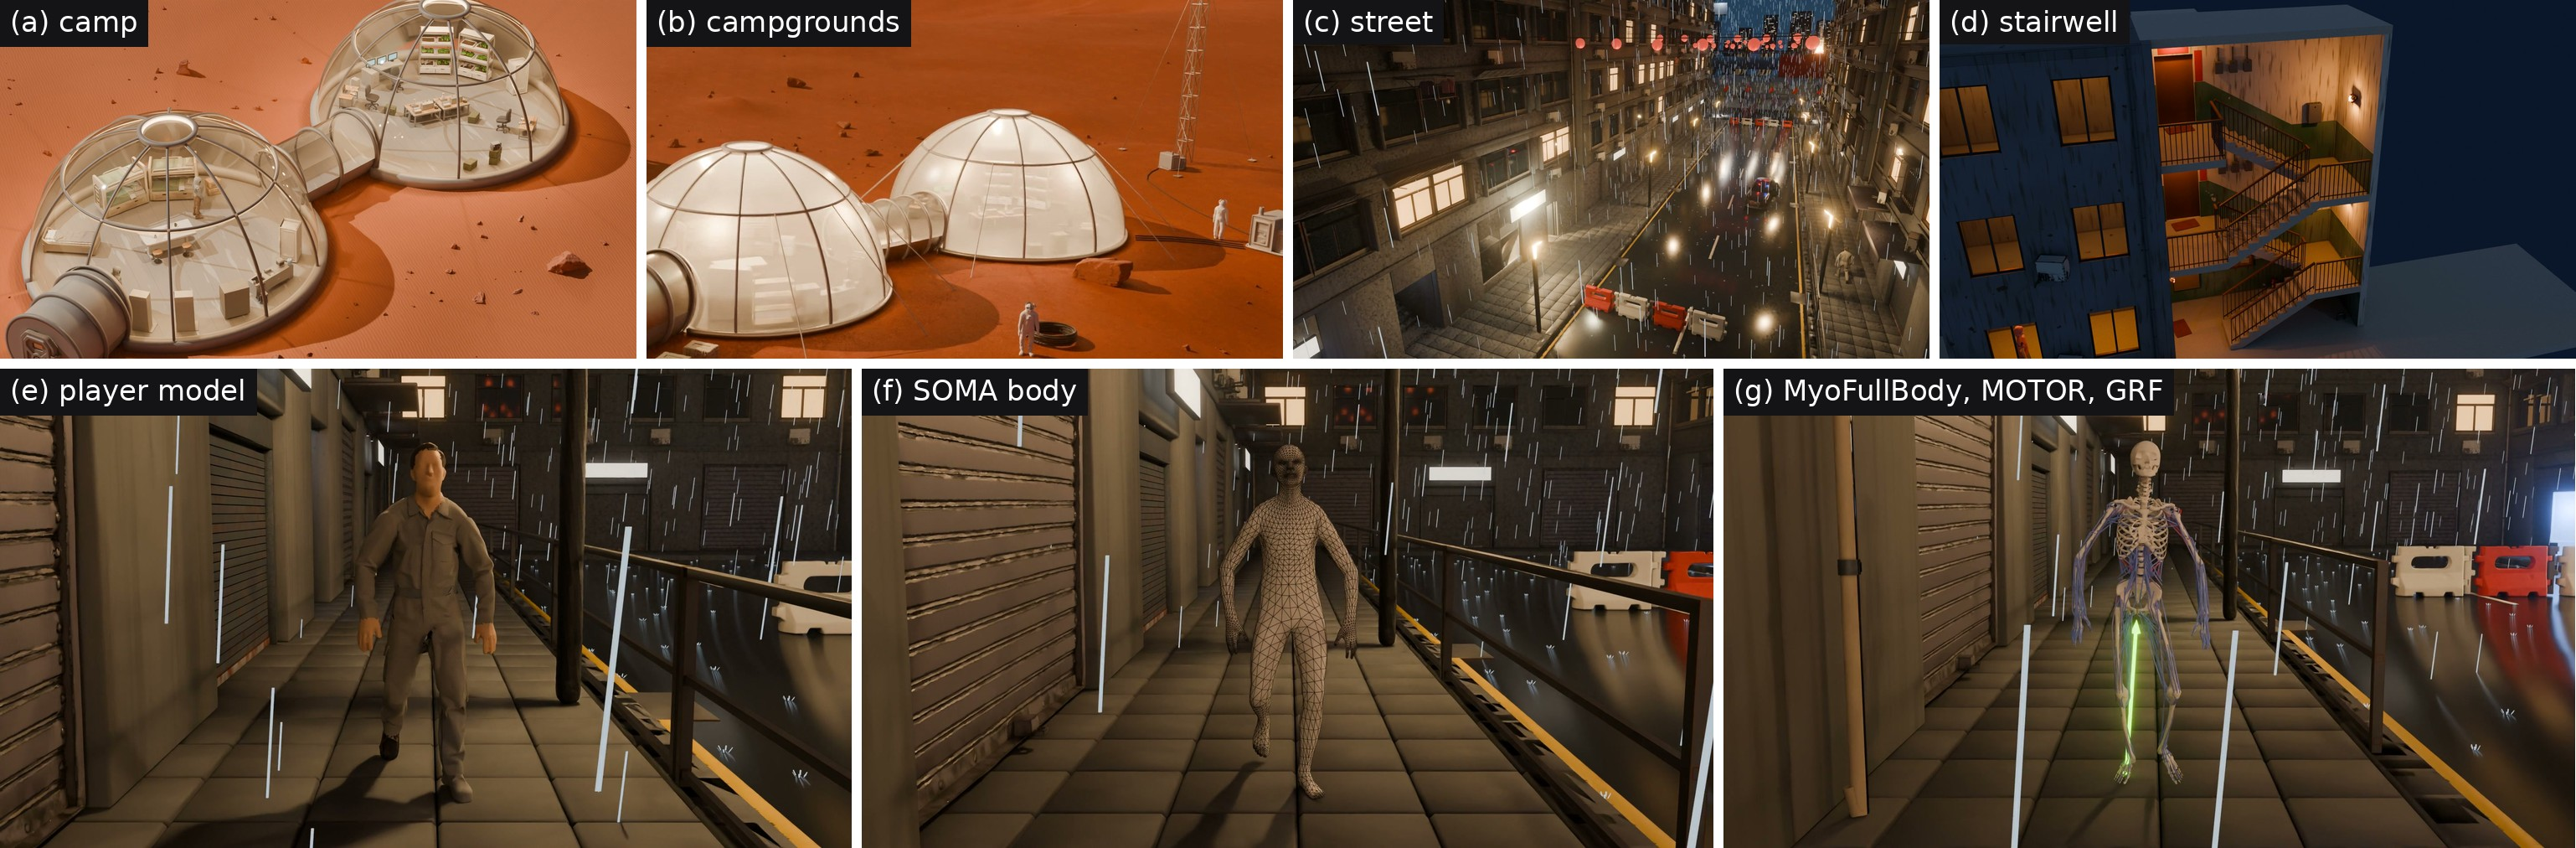
\includegraphics[width=1\linewidth,height=\textheight,keepaspectratio,alt={(a)--(d) Opening frames of the four released films: camp, campgrounds (cropped), street and stairwell. (e)--(g) One walker in the street film, peeled from its player model to its SOMA body to its MyoFullBody sim body solved by MOTOR, with the vertical ground reaction force drawn at the stance foot.}]{figures/results.jpg}
\caption{(a)--(d) Opening frames of the four released films: camp, campgrounds (cropped), street and stairwell. (e)--(g) One walker in the street film, peeled from its player model to its SOMA body to its MyoFullBody sim body solved by MOTOR, with the vertical ground reaction force drawn at the stance foot.}
\end{figure}

SCORE first derived each scene from its concept through model readings, written plans and generated shells. Over all 26 places of a first environment, reviewing vision-model agents scored it a mean of 2.2 out of 10 against the concepts, with wrong shells in 18 places and objects dropped or doubled in 22, and eight rounds of fixes did not improve it. The layered method replaced it for four places: camp, campgrounds, stairwell and street (Figure 2).

All four pass the place check without a fault, on 711, 1046, 61 and 890 objects. The builder's own critic scored their concept views 7, 7, 4 and 6 out of 10, the old method's reviewers 2, 4, 1 and 1; with different judges and no human rating, the two sets are not directly comparable. TRELLIS.2 was judged better than the earlier route on five of six camp props and runs in 170 to 220 s per model on a local 16 GB card at no rental cost, against about EUR 0.22 before. First film renders cost about EUR 17 on rented cards, the published re-renders EUR 45 to 50.

The people are the weakest layer. In the first films of 17 November, twelve of thirteen walkers stayed within 6.8 cm of their routes, but no sim body passed the residual check over a whole clip: the best street walker met the force limit (13.2 N against 15.2 N) but not the moment limit (13.4 N m against 7.4 N m), and the stairwell woman peaked at 1,368 N against 15 N while sinking about 17 cm. The published re-films still fail it at every walker's peaks. The scenes are not photorealistic: surfaces are clean and pale, kits repeat and signs are illegible. The settle runs under Earth's gravity even on Mars, and the check judges rest, not function.

A revised foot contact in MOTOR lowered per-foot vertical ground reaction force error in all four motions of 13 trials but raised the pelvis residual moment by 1.5 to 6 N m \citep{motorcontact}, so the residual limits remain open work. Articulated UsdPhysics joints would make doors and machines operable, and the settle should take each plot's own gravity. The larger step is a whole environment judged by human raters. Coding agents placed every object through the framework's commands, judged the renders and wrote most of the code; the creator's locks and decisions were his own.
